\chapter{Methodologies}

\label{chapter:methodologies}

\section{FMTOD data set}

\citet{schuster-etal-2019-cross-lingual} originally released the Facebook Multilingual Task Oriented Dialog (FMTOD) data set to encourage research in cross-lingual transfer learning for Natural Language Understanding (NLU) tasks; specifically from from high-resource to low-resource languages. The authors released the FMTOD data set with English as the high-resource language with $\sim$43k annotated sentences, and Spanish and Thai as low-resource languages with a total of $\sim$14k sentences. Furthermore, they streamlined the data set on two key tasks; namely intent detection and textual slot filling. In this thesis, we focus solely on the English language intent detection task in the FMTOD data set. This intent detection task entails a multi-label sequence classification task with a total of 12 classes from alarm, reminder and weather-related domains.

\subsection{Motivation}

We chose to work with the FMTOD data set since it is both a recently released and well-studied data set \citep{schuster-etal-2019-cross-lingual,zhang2019joint,zhang2020intent,ren2020intention}. We focus on the English language intent classification task since it is a relatively straightforward task which allows us to place a greater focus on performance and explainability. Furthermore, the English language subset entails the highest resources in the FMTOD data set. Finally, we find the FMTOD data set's intent detection classification especially attractive because it allows us to test the SoPa++ model on a multi-class NLU problem; which is significantly different from the focus on binary classification sentiment detection tasks in SoPa \citep{schwartz2018sopa}.

\subsection{Preprocessing}

We enumerate our preprocessing steps below:

\begin{enumerate}{}
  \item Similar to \citet{schwartz2018sopa}, we convert all FMTOD text samples to a lowercased format. This assists in simplifying the data set further.
  \item Next, we search through the pre-provided training, validation and test data partitions to remove duplicates within each partition.
  \item Finally, we remove data duplicates which overlap between partitions. During this step, we do not remove any cross-partition duplicates from the test set in order to keep it as similar as possible to the original test partition. This comes into importance later when we compare performance evaluations on the test set with other studies.
\end{enumerate}

Many of the duplicates observed were already present in the original FMTOD data set, with additional duplicates being created from the initial lowercasing step. After preprocessing, we obtain a lowercased variant of the FMTOD data set with strictly unique data partitions. In the next section, we describe the summary statistics of the preprocessed FMTOD data set.

\begin{figure}[t]
  \centering
  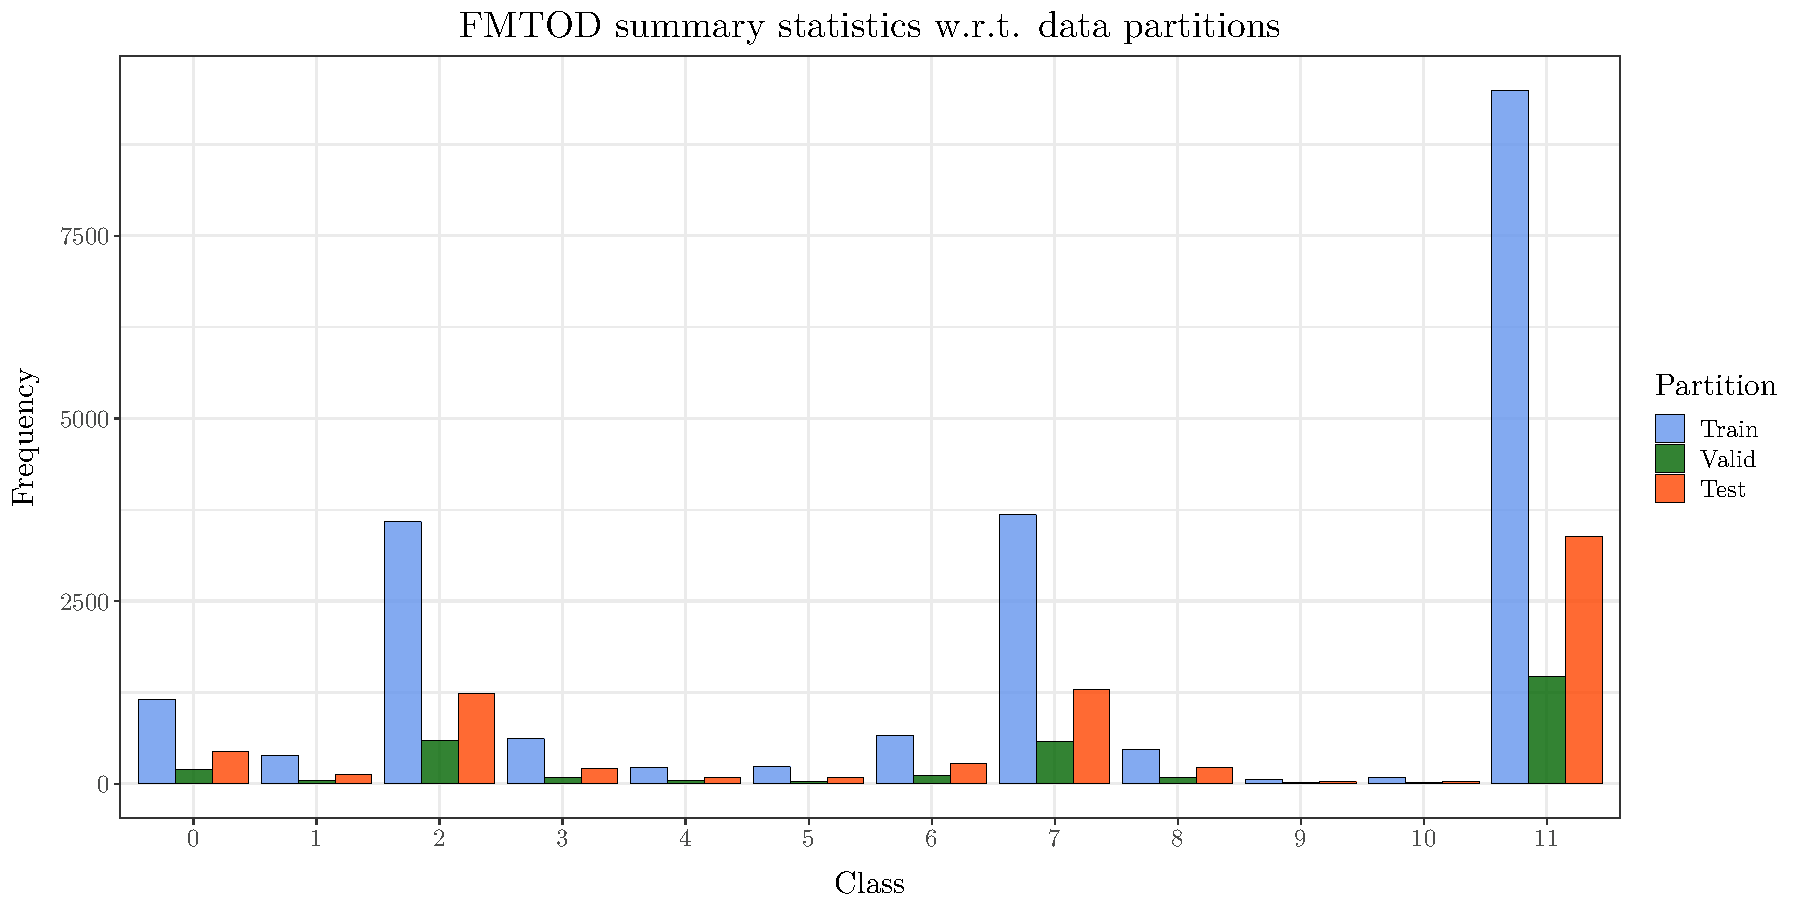
\includegraphics[width=14cm]{pdfs/generated/fmtod_summary_statistics.pdf}
  \caption{Data distribution of the preprocessed FMTOD data set grouped by classes and partitions}
  \label{fig:fmtod}
\end{figure}

\begin{table}[t!]
  \centering
  \begin{tabular}{llllll}
    \toprule
    Class & Description & Train & Validation & Test & Combined \\
    \midrule
    0 & \texttt{alarm/cancel\_alarm} & 1157 & 190 & 444 & 1791 \\
    1 & \texttt{alarm/modify\_alarm} & 393 & 51 & 122 & 566 \\
    2 & \texttt{alarm/set\_alarm} & 3584 & 596 & 1236 & 5416 \\
    3 & \texttt{alarm/show\_alarms} & 619 & 83 & 212 & 914 \\
    4 & \texttt{alarm/snooze\_alarm} & 228 & 49 & 89 & 366 \\
    5 & \texttt{alarm/time\_left\_on\_alarm} & 233 & 30 & 81 & 344 \\
    6 & \texttt{reminder/cancel\_reminder} & 662 & 114 & 284 & 1060 \\
    7 & \texttt{reminder/set\_reminder} & 3681 & 581 & 1287 & 5549 \\
    8 & \texttt{reminder/show\_reminders} & 474 & 82 & 217 & 773 \\
    9 & \texttt{weather/check\_sunrise} & 63 & 13 & 25 & 101 \\
    10 & \texttt{weather/check\_sunset} & 88 & 11 & 37 & 136 \\
    11 & \texttt{weather/find} & 9490 & 1462 & 3386 & 14338 \\[5pt]
    \hline \hline \\[-10pt]
    $\Sigma$ & \textemdash & 20672 & 3262 & 7420 & 31354 \\
    \bottomrule\\
  \end{tabular}
  \caption{Frequency of the preprocessed FMTOD data set classes grouped by partitions; $\Sigma$ signifies the cumulative frequency in each data partition}
  \label{tab:fmtod}
\end{table}

\subsection{Summary statistics}

Figure \ref{fig:fmtod} shows the summary statistics of the preprocessed FMTOD data set grouped by classes and data set partitions. Similarly, Table \ref{tab:fmtod} shows the same summary statistics in a tabular form with explicit frequencies. Based on the summary statistics, we can observe that the preprocessed FMTOD data set is significantly imbalanced with $\sim$45$\%$ of samples falling into Class 11 alone. We take this observation into consideration in later sections and apply fixes to mitigate this data imbalance. In addition, we observe that input sentences in the preprocessed FMTOD data set are generally short; with a mean input token count of 7.7 and a standard deviation of 2.5 tokens.

\subsection{Performance range}

Several studies have optimized deep learning models on the FMTOD English language intent classification task using a variety of models from CNNs and BiLSTMs to BERT and XLM-RoBERTa \citep{schuster-etal-2019-cross-lingual,zhang2019joint,zhang2020intent,ren2020intention}. The general accuracy range for the English language FMTOD intent classification task from the aforementioned studies is 96$\%$ to 99$\%$. 

%%% Local Variables: 
%%% mode: latex
%%% TeX-master: "main"
%%% End: 